\chapter{Introduction}

\hl{cite} \cite{ebner2008generalized}: using a solver for optimal instruction selection

A \gls{compiler}
  is a tool which
  converts from one representation
  to another---%
  usually, from a
  higher-level,
  human-readable representation
  to a lower-level,
  machine-readable representation.
A classic example
  is the clang compiler
  from the LLVM suite,
  which
  compiles programs written in 
  processor-independent C code
  into processor-specific
  machine code,
  which the hardware understands how
  to execute:
\begin{figure}[!h]
\centering
\begin{tikzpicture}
  \draw[inner sep = 5pt] (0,0) node [draw, thin] (c) \bgroup%
\begin{minipage}{10em}
\begin{minted}[fontsize=\small,baselinestretch=1]{c}
int square(int num) {
    return num * num;
}
\end{minted}
\end{minipage}
  \egroup;
  
\draw[inner sep = 5pt] (8.75,0) node [draw, thin] (asm) \bgroup%
\begin{minipage}{7em}
\begin{minted}[fontsize=\small,baselinestretch=1]{asm}
square:
 imul edi, edi
 mov eax, edi
 ret
\end{minted}
\end{minipage}
  \egroup;

\draw[inner sep = 5pt] (4.5,0) node [draw, thin] (compiler) {clang};

  \draw[->, very thick] (c) edge (compiler) (compiler) edge (asm);
\end{tikzpicture}
\caption{clang compiling high-level C code to target-specific x86 assembly.}
\label{fig:clang-c-to-x86}
\end{figure}

\noindent
In this case,
  clang is generating code 
  for an x86 processor;
  we refer to 
  the platform
  which the compiler is compiling for
  as the \gls{target}.
Though compilers perform many target-agnostic
  transformations and optimizations
  (modifications of the high-level code
    which are useful regardless of the target),
  a compiler's fundamental purpose
  is to produce a program
  in the target's language.
The portion of the compiler
  which handles target-specific optimizations
  and code generation is called the
  \gls{compilerbackend}---%
  for example,
  it is clang's x86 backend which is responsible for
  performing x86-specific optimizations
  and eventually producing
  x86 assembly code.
Compiler backends will be the focus
  of this dissertation;
  we will largely ignore other compiler components
  (i.e.~frontends and target-independent optimizations).

Throughout this intro,
  we will use three different compilers
  as our running examples.
As we have already seen, we will
  consider the
  general-purpose C compiler
  clang
  as our ``gold standard'' example
  of a commonly-known
  and understood compiler.
However, we will also consider
  two compilers from more specialized
  domains,
  which will be key to
  \cref{part:glenside-and-3la}
  and
  \cref{part:lakeroad}
  of this dissertation,
  respectively.
First,
  the TVM compiler~\cite{tvm,chen2018tvm},
  which will be a main focus
  of \cref{part:glenside-and-3la},
  is a compiler for deep learning
  programs
  which compiles code written in a
  high-level
  Python
  \gls{dsl}
  into optimized code
  for CPUs, GPUs,
  and custom accelerators.
Second,
  the open-source \gls{hardwaresynthesis}
  tool Yosys
  is a compiler for hardware designs,
  and will be a focus of
  \cref{part:lakeroad}.

Compiler backends are composed
  of multiple stages,
  and each stage is implemented with
  one or a number of core
  \textbf{algorithms.}
A key stage in clang's x86 backend
  when compiling our example in
  \cref{fig:clang-c-to-x86}
  is
  \textit{instruction selection,}
  \hl{glossary}
  in which clang decides how to implement
  each operation in the C program
  using actual instructions
  provided by the processor.
It is in this stage, for example, 
  where clang decides to
  implement
  C's \texttt{*} operator
  using x86's
  \texttt{imul} instruction.
clang does this using
  an \textit{instruction selection}
  algorithm~\cite{llvminstructionselection}.

\begin{figure}
\centering
\begin{tikzpicture}
  \draw[inner sep = 5pt] (0,0) node [draw, thin] (c) \bgroup%
\begin{minipage}{11em}
\begin{minted}[fontsize=\small,baselinestretch=1]{python}
nn.conv2d(data, weight, 
 padding=[1, 1, 1, 1], 
 channels=16, 
 kernel_size=[3, 3])
\end{minted}
\end{minipage}
  \egroup;
  
\draw[inner sep = 5pt] (8.75,0) node [draw, thin] (asm) \bgroup%
\begin{minipage}{14em}
\begin{minted}[fontsize=\small,baselinestretch=1]{python}
with T.attr("VTAPushGEMMOp"):
 for j_init in range(14):
  T.tir.vta.uop_push(...)
\end{minted}
\end{minipage}
  \egroup;

\draw[inner sep = 5pt] (4.5,0) node [draw, thin] (compiler) {TVM};

  \draw[->, very thick] (c) edge (compiler) (compiler) edge (asm);
\end{tikzpicture}
\caption{Tensorizing a 2D convolution to VTA~\cite{moreau2018vta} accelerator calls.
\hl{fix this figure and tech mapping figure, they look wonky and they're not in the right places}}
\label{fig:intro:tensorization}
\end{figure}


\begin{figure}[]
\centering
\begin{tikzpicture}
  \draw[inner sep = 5pt] (0,0) node [draw, thin] (c) \bgroup%
\begin{minipage}{16em}
\begin{minted}[fontsize=\small,baselinestretch=1]{verilog}
module add_mul_add(input a,b,c,d,
  output o);
 assign out <= ((d + a) * b) + c;
endmodule
\end{minted}
\end{minipage}
  \egroup;
  
\draw[inner sep = 5pt] (8.75,0) node [draw, thin] (asm) \bgroup%
\begin{minipage}{11em}
\begin{minted}[fontsize=\small,baselinestretch=1]{verilog}
DSP48E2 #(
  .ACASCREG(32'd1), ...
) DSP48E2_0 (
  .A(a), ...
);
\end{minted}
\end{minipage}
  \egroup;

\draw[inner sep = 5pt] (4.5,0) node [draw, thin] (compiler) {Yosys};

  \draw[->, very thick] (c) edge (compiler) (compiler) edge (asm);
\end{tikzpicture}
\caption{Technology mapping a high-level
  hardware design
  to an instantiation of a specific 
  hardware primitive.}
\label{fig:intro:techmapping}
\end{figure}


Our other two compiler examples,
  TVM and Yosys,
  also rely on a few core algorithms
  to implement their backends.
TVM, for example, implements a step
  called 
  \textit{tensorization}~\cite{tvmtensorization},
  which, among other things, maps high-level 
  \glspl{mlkernel}
  to target-specific implementations,
  including invocations
  of specialized hardware.
\Cref{fig:intro:tensorization}
  shows an example of tensorizing 
  a 2-dimensional convolution
  to general matrix multiplication (GEMM) instructions
  for a specific accelerator backend, VTA.
Similarly,
  a core step in hardware compilation
  for
  Yosys and other hardware synthesis tools \hl{glossary}
  is \textit{technology mapping,} \hl{glossary}
  in which the tool determines
  how to implement the high-level
  hardware design
  using the hardware primitives
  available on the hardware
  platform.
An example of technology mapping is shown in
  \cref{fig:intro:techmapping},
  in which a high-level, architecture-independent
  hardware module 
  is implemented using an
  architecture-specific hardware primitive
  (in this case, a DSP48E2 primitive
    present on Xilinx FPGAs).
Both tensorization
  and technology mapping
  will be key focuses of this dissertation,
  in \cref{part:glenside-and-3la,part:lakeroad}
  respectively.

To implement their core algorithms,
  compiler backends 
  employ \textbf{models} of hardware.
% Whether or not they are apparent,
%   built into every compiler backend
%   are \textbf{models}
%   of the target platform.
clang's instruction selection algorithm,
  for example,
  directly utilizes a model
  of the x86 architecture's
  instructions
  to determine what instructions
  are available for use.
The model is explicit,
  built into clang's x86 backend itself.
The following snippet is
  taken from the x86 instruction model,
  and is the declaration
  of the \texttt{imul} instruction
  used to implement our \texttt{square}
  function above:
  
\vspace{4mm}
\begin{figure}[H]
    \centering
%defm MUL : Mul<0xF7, "mul", MRM4r, MRM4m, mul>;
\begin{minted}[baselinestretch=1]{cpp}
defm IMUL : Mul<0xF7, "imul", MRM5r, MRM5m, null_frag>;
\end{minted}
\caption{
Declaration of x86's
  \texttt{imul}
  instruction in LLVM's x86 
  backend~\cite{llvmx86tablegen}.
}
    \label{fig:intro:llvm-tablegen}
\end{figure}


Not all models within compilers
  are made the same, however.
To contrast the explicit model in
  \cref{fig:intro:llvm-tablegen},
  consider this snippet from Yosys's technology mapper
  for Xilinx FPGAs:

\vspace{4mm}

% Lastly, as an example from
%   yet another different domain,
%   this code snippet~\cite{yosysxilinxpmgen}
%   comes from
%   the open source hardware synthesis tool 
%   Yosys's~\cite{wolf2013yosys}
%   \texttt{pmgen} framework:

\begin{figure}[H]
    \centering
\begin{minted}[baselinestretch=1]{c}
subpattern in_dffe
arg argQ clock
code
  dff = nullptr;
  if (argQ.empty())
    reject;
  for (const auto &c : argQ.chunks()) {
    if (!c.wire)
      reject;
    ...
\end{minted}
    \caption{
Snippet of code
  from Yosys's pmgen framework~\cite{yosysxilinxpmgen}
  attempting to map hardware designs
  to specific hardware primitives.
    }
    \label{fig:intro:yosys-pmgen}
\end{figure}

% This code
%   captures a model of a specific hardware platform's functionality;
%   specifically, it checks whether
%   there is a \textit{D flip-flop}
%   (a specific hardware primitive)
%   on the input of a hardware module,
%   and folds it in to a larger module
%   if so
%   (which is omitted).

\noindent
This code is an imperative pattern matching
  algorithm
  written in Yosys's pmgen \gls{dsl}
  which searches for a specific pattern 
  in the hardware design.
Unlike \cref{fig:intro:llvm-tablegen},
  which is an explicit hardware model
  \textit{used by} clang's instruction selector algorithm,
  the above example is \textit{both} algorithm
  \textit{and} model:
  encoded \textit{implicitly}
  within this algorithm
  is a model of the underlying hardware.%
\footnote{In fact, it would be quite difficult
  to build a compiler
  \textit{without} encoding some kind 
  of model of the underlying hardware.
That is, any compiler which generates code
  for a hardware target
  will encode facts about the hardware
  which amount to a model of the hardware,
  however implicit.}
Soon, I will argue why this method
  of entwining algorithm
  and model
  is disadvantageous;
  before I do that, however,
  I will introduce some terminology
  to make it easier to discuss 
  the properties
  of algorithms and models.

To better discuss compiler backends'
  algorithms
  and the hardware models on which
  they depend,
  I introduce two terms:
  \textit{model explicitness}
  and
  \textit{algorithm adaptability.}
  
\paragraph{Model explicitness.}
% I claim that it would be difficult
%   to build a compiler backend
%   without encoding some sort of model
%   of the target
%   into the backend;
Model explicitness
  captures
  how overtly
  a model is encoded
  into a compiler backend.
For example,
  \cref{fig:intro:llvm-tablegen}
  presents an overt, 
  explicit model of hardware
  in the form of a list
  of instructions
  implemented on x86.
In contrast,
  \cref{fig:intro:yosys-pmgen}
  presents an implicit model
  embedded within a pattern matching
  algorithm.
We consider
  \cref{fig:intro:llvm-tablegen} more explicit
  as the model is easier to identify
  and interpret.
Model explicitness is also highly correlated
  to whether or not the model
  is captured in a \textit{declarative} form---%
  that is, in a non-executable format,
  such as the static list of instructions
  in \cref{fig:intro:llvm-tablegen}---%
  or in an \textit{imperative} form
  such as the executable pattern matching
  algorithm in \cref{fig:intro:yosys-pmgen}.

\paragraph{Algorithm adaptability.}
Algorithm adaptability captures the
  ability of a particular compiler backend
  algorithm
  (e.g.~an instruction selection
    algorithm
    or a technology mapping algorithm)
  to adapt
  to new hardware
  with minimal modification.
For example,
  because
  clang's instruction selection algorithm
  reads its instructions from
  declarative models
  such as the one presented in
  \cref{fig:intro:llvm-tablegen},
  it can easily adapt to new instructions
  and hardware targets
  by simply being supplied
  a new list of instructions~\cite{llvminstructionselection}.
Yosys's technology mapping algorithm
  presented in 
  \cref{fig:intro:yosys-pmgen},
  on the other hand,
  encodes a model of the 
  target FPGA
  implicitly within the algorithm;
  thus, adapting it to a new FPGA
  would involve entirely rewriting
  the algorithm.

\vspace{10mm}

  
\begin{figure}
    \centering
    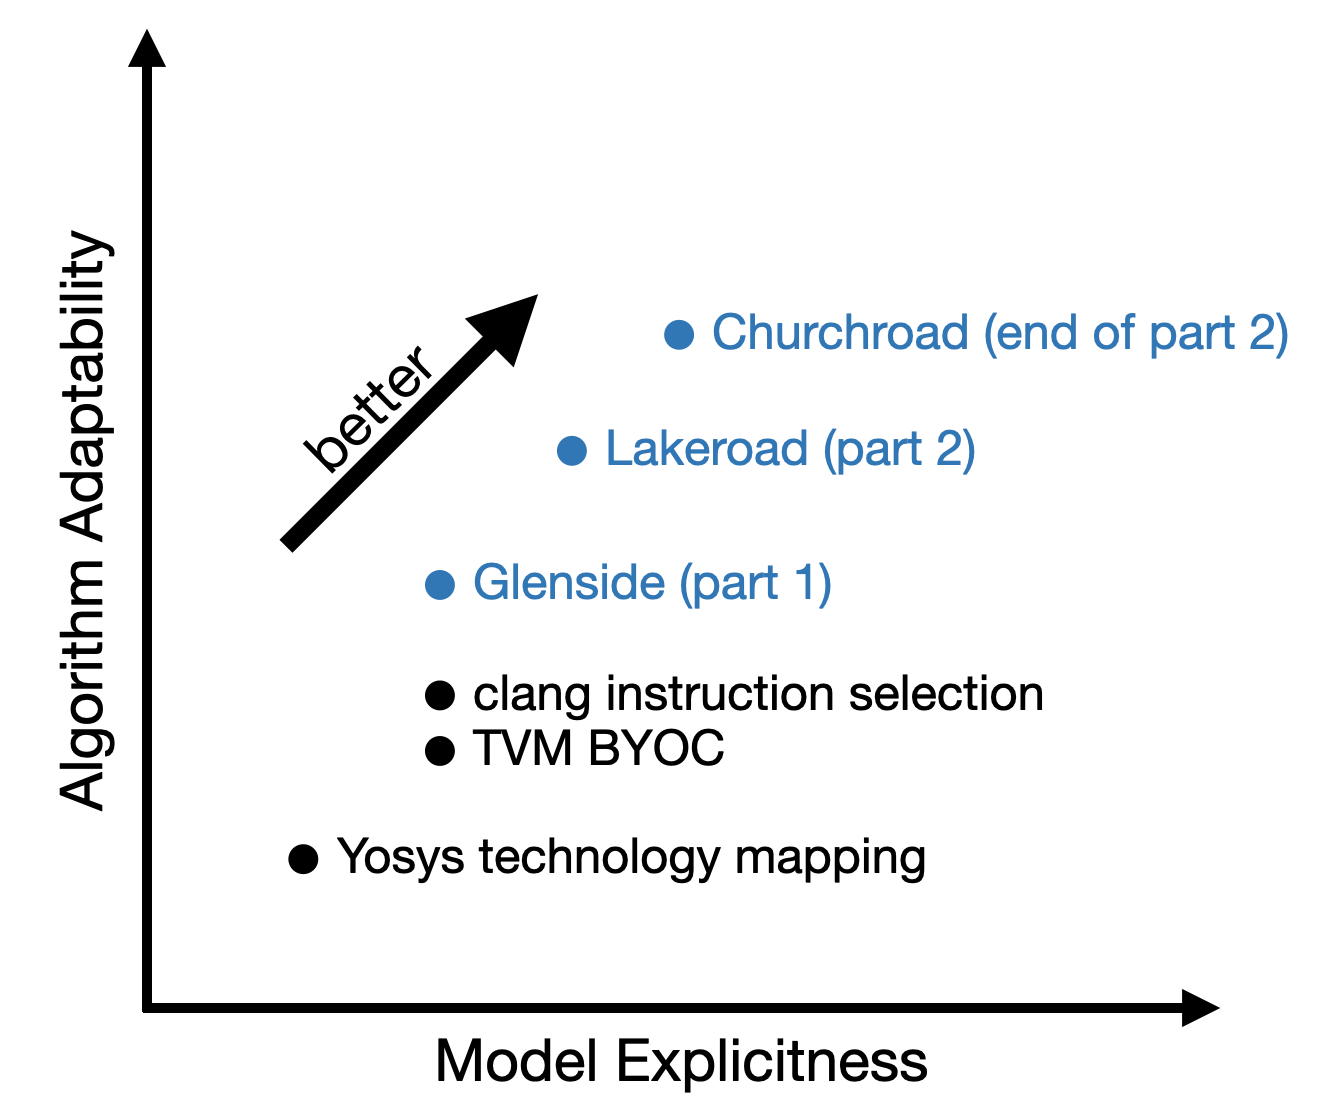
\includegraphics[width=.7\textwidth]{intro-figures/model-alg-spectrum-keynote.png}
    \caption{
A visualization of where various compiler backend
  components
  fall
  on the model explicitness--algorithm automation
  spectrum.
Blue dots represent contributions of this
  dissertation.
    }
    \label{fig:intro:model-alg-spectrum}
\end{figure}



Now that we've introduced these terms,
  let's 
  reconsider the two examples we have discussed so far:
  clang's instruction selector
  and Yosys's technology mapper.
clang's instruction selector is powered by
  an \textit{explicit} model of the x86 ISA,
  part of which is presented in
  \cref{fig:intro:llvm-tablegen}.
Furthermore, its underlying algorithm
  is \textit{adaptable} to new models;
  the user simply needs to update
  the model, and the algorithm will adapt.
On the other hand,
  Yosys's technology mapper utilizes
  \textit{implicit} models,
  and its algorithm is \textit{inflexible}.
To visualize this, we
  we plot Yosys's techology mapper
  and clang's instruction selector
  on a 2D plane
  with model explicitness on the horizontal axis
  and algorithm adaptability on the vertical axis,
  shown in \cref{fig:intro:model-alg-spectrum}.
Yosys's technology mapper,
  being built upon implicit models
  and inflexible algorithms,
  is towards the bottom left.
Meanwhile, clang's instruction selection
  is further up and to the right.

% \hl{move?}
% Note that algorithm adaptability
%   and model explicitness
%   are often intertwined ideas.

\textbf{The core claim of this dissertation,
  put informally,
  is that pushing up
  and to the right
  on our model explicitness--algorithm adaptability
  spectrum (\cref{fig:intro:model-alg-spectrum})
  produces better compiler backends.}
  % that is,
  % using
  % more adaptable algorithms
  % and more explicit models
  % leads to better compiler backends.
I specifically focus on
  using adaptable automated reasoning algorithms
  to \textit{automatically generate}
  compiler backends
  from explicit, formal models of hardware.
I claim there are three primary classes
  of improvements
  from automatically generating 
  compiler backends:
  correctness,
  optimization,
  and development time improvements.
  
Next, I present my formal
  thesis statement.
Afterwards, I will break down the statement
  and discuss each part.

\hl{"all models are wrong, some are useful"}

\mdfsetup{
    frametitle={\colorbox{white}{\space{Thesis Statement}\space}},
    innertopmargin=10pt,
    frametitleaboveskip=-9,
    frametitlealignment=\center
    }
\begin{mdframed}
% Defined in toplevel imports-and-macros.tex
\mythesis
\end{mdframed}

\vspace{10mm}

I will now explain and define
  the individual components
  of this thesis.
I will use a set of five keywords
  to refer back to 
  to the primary components of my
  thesis statement:
  its two ``inputs'',
  \cref{thesis:algorithms} and
  \cref{thesis:models},
  and its three ``outputs'',
  \cref{thesis:optimizations},
  \cref{thesis:correctness}, and
  \cref{thesis:devtime}.

\paragraph{Automatically generating compiler 
  backends.}
At the highest level,
  my thesis advocates for
  automatically generating compiler backends.
By this, I mean
  utilizing automated reasoning techniques
  to automatically implement
  compiler backend tasks like
  tensorization in ML compilers
  and technology mapping in FPGA compilers.
At the highest level,
  automatically generating compiler backends
  takes the form of
  feeding
  a hardware model
  into an algorithm,
  allowing the algorithm
  to reason about the hardware.
\hl{weak}
I break down the automated generation
  of compiler backends
  into two primary design decisions:
  choosing an automated reasoning algorithm
  (which we refer to via
    \cref{thesis:algorithms})
  and choosing the formal hardware models
  to feed into the algorithms
  (which we refer to via
    \cref{thesis:models}).
I thus consider   
  the
  \cref{thesis:algorithms}
  and
  \cref{thesis:models}
  as ``inputs''
  or the independent variables
  in my research.
In \cref{part:glenside-and-3la,part:lakeroad},
  I will show how
  different choices of 
  \cref{thesis:algorithms}
  and
  \cref{thesis:models}
  produce different results.
I will now discuss
  each of these inputs
  in more detail.

\paragraph{\cref{thesis:algorithms}.}
\cref{thesis:algorithms}
  refers
  to the automated reasoning algorithms
  we use
  to automatically generate our backends.
In
  \cref{part:glenside-and-3la},
  we focus on an algorithm called
  equality saturation;
  in
  \cref{part:lakeroad},
  we focus on an algorithm called
  program synthesis.

\paragraph{\cref{thesis:models}.}
\cref{thesis:models}
  refers to the hardware models
  which the automated reasoning algorithms
  consume
  to generate the compiler backend.
In \cref{part:glenside-and-3la},
  our models take the form
  of program rewrites,
  capturing the high-level 
  functional behavior
  of hardware accelerators.
In \cref{part:lakeroad},
  we directly utilize
  vendor-provided
  Verilog simulation models.

\vspace{10mm}

In my thesis statement,
  I claim that automatically generating
  compiler backends
  benefits compiler
  \cref{thesis:optimizations},
  \cref{thesis:correctness}, and
  \cref{thesis:devtime}.
We consider these the ``outputs''
  or dependent variables
  in our experiments
  in \cref{part:glenside-and-3la,part:lakeroad}.
I now describe each in detail.

\paragraph{\cref{thesis:optimizations}.}
A key task of a compiler backend
  is to utilize the target hardware
  efficiently
  to produce optimized programs.
Compiler backends which rely on poor,
  implicitly encoded models
  and inflexible algorithms
  leave key optimizations on the table.
\hl{would be nice to show that automated methods have clearly shown
  to be superior when it comes to optimizing programs.
  STOKE, AutoTVM, synthesis in general, ML guided?}

\paragraph{\cref{thesis:correctness}.}
Compiler backends are expected to produce correct code.
However,
  backends which are built on
  implicit models of hardware
  which are deeply integrated into
  the algorithms themselves
  can have hard-to-find bugs.
A cleaner division between hardware model
  and algorithm
  makes it easier to find bugs on either side.
Furthermore, many of the
  more adaptable algorithms
  I advocate for in this dissertation
  (equality saturation, program synthesis)
  have open-source, highly-used, well-tested
  implementations
  which are likely more trustworthy
  than a hand-implemented
  algorithm used only within
  a single compiler backend.

\paragraph{\cref{thesis:devtime}.}
And lastly,
  more explicit models
  and more adaptable algorithms
  can ease compiler development.
Implicit models,
  especially models deeply integrated
  into the algorithms themselves
  (such as the Yosys example
    in \cref{fig:intro:yosys-pmgen})
  are generally harder to comprehend
  and thus harder to update.
Understanding implicit,
  imperative models
  is often more challenging
  than understanding explicit,
  declarative models.
More flexible algorithms
  reduce development time in a number of ways.
First, the algorithms
  this dissertation promotes
  all have free-to-use open source 
  implementations,
  thus alleviating the need
  for the compiler engineer
  to write their own algorithm by hand.
Second, the greater flexibility
  of the algorithms
  allows them to adapt to new
  hardware
  with less engineering effort.

\vspace{10mm}

I will demonstrate this thesis
  in two parts.
These parts are visualized on
  our model explicitness--algorithm adaptability
  spectrum in
  \cref{fig:intro:model-alg-spectrum}.
In \cref{part:glenside-and-3la},
  I introduce Glenside,
  which demonstrates how
  a more adaptable algorithm
  can increase a compiler's
  ability to offload operations
  to machine learning accelerators.
As is shown in
  \cref{fig:intro:model-alg-spectrum},
  \cref{part:glenside-and-3la}
  only pushes along one axis 
  of our spectrum.
In \cref{part:lakeroad}, I
  more fully realize
  my thesis statement
  via Lakeroad:
  a technology mapper for FPGAs
  which utilizes both more
  adaptable algorithms
  and
  more explicit models.
Glenside and Lakeroad
  both demonstrate
  how,
  by automatically generating
  portions of compiler backends
  using more adaptable algorithms
  and more explicit models of hardware,
  we we improve their
  optimization ability and
  correctness, while
  easing development effort.

\hl{we still don't land the intro very strongly}

\hl{STUFF BELOW THIS LINE IS ROUGH}

\hl{Hardware models are pervasive:}
The reliance of modern compilers
  on \textit{implicit} models is truly odd, 
  given that
  explicit, formal models
  of the target hardware
  almost certainly exist
  in all cases.
In fact, nearly all hardware design
  \textit{begins} from the construction
  of these models
  at a high level of abstraction;
  the bulk of the hardware design process
  is building low-level implementations
  of the high-level specification,
  and verifying the implementation
  is equivalent.
Thus, \textbf{there is wealth
  of explicit, formal models of hardware
  which could be used
  instead of implicit models.}
\hl{examples of explicit hw models? alistair's work?
should probably go into a later paragraph}
\hl{maybe something about declarative programming being good?
a trend towards declarative programming?}

\hl{Hardware models are prime for use with automated tools:}
Furthermore, 
  there exist plenty of automated
  tools
  which deal with
  these formal models.
Oddly, though,
  many of these tools
  are concerned only with
  what happens \textit{after}
  compilation.
\hl{cite zach sisco latte, he says this directly}
That is, the formal models
  of hardware
  are used to check that 
  the compiled program is correct.
Why not instead
  just ensure
  that you can't compile an incorrect
  program?

\hl{The models are more correct:}
Lastly, and perhaps most importantly,
  these explicit models
  are perhaps \textit{more correct}
  than any implicit, handwritten models
  that could be written,
  as in many cases, these models
  are the \textit{ground truth.}

Furthermore, it is our position that
  \textbf{recent advances
  in programming languages
  make automated compiler construction
  feasible.}
The idea of automatically generating
  compiler backends is not new:
  previous work includes
  synthesizing instruction selectors%
  ~\cite{buchwald2018synthesizing,dias2010automatically,brandner2007compiler,daly2022synthesizing}
  and code generators~\cite{leupers1997retargetable,brandner2013automatic},
  among other work.
However, much of this work
  is a decade old, if not more,
  and does not benefit from
  advances in
  languages and type systems
  for hardware~\cite{durst2020type,nigam2023modular,nigam2020predictable},
  equational reasoning via equality saturation~\cite{tate2009equality,willsey2021egg},
  program synthesis~\cite{solar2008program,torlak2013growing},
  and machine learning for program generation~\cite{alon2019code2vec,austin2021program}.Furthermore, it is our position that
  \textbf{recent advances
  in programming languages
  make automated compiler construction
  feasible.}
The idea of automatically generating
  compiler backends is not new:
  previous work includes
  synthesizing instruction selectors%
  ~\cite{buchwald2018synthesizing,dias2010automatically,brandner2007compiler,daly2022synthesizing}
  and code generators~\cite{leupers1997retargetable,brandner2013automatic},
  among other work.
However, much of this work
  is a decade old, if not more,
  and does not benefit from
  advances in
  languages and type systems
  for hardware~\cite{durst2020type,nigam2023modular,nigam2020predictable},
  equational reasoning via equality saturation~\cite{tate2009equality,willsey2021egg},
  program synthesis~\cite{solar2008program,torlak2013growing},
  and machine learning for program generation~\cite{alon2019code2vec,austin2021program}.

In this dissertation,
  I present the case for
  automatically generating compiler backends
  from
  formal models of hardware.
I apply this technique
  to two separate domains:
  (1) compilation for
  domain-specific 
  deep learning accelerators,
  and
  (2) hardware compilation 
  (or \textit{synthesis})
  for Field-Programmable
  Gate Arrays (FPGAs).
In both of these cases,
  I show how
  automatically generating
  a portion of the compiler backend
  leads to increased correctness,
  greater extensibility,
  and more powerful automated optimization.

In the first part,
  I demonstrate
  how explicit,
  handwritten
  models of hardware,
  captured as
  \textit{rewrites,}
  can be used 
  to automatically implement
  ``instruction selection''
  for machine learning
  accelerators.

In the second part,
  I apply this thesis
  even more literally, by using
  formal models of hardware
  not written by us,
  but found in the wild,
  to build a compiler
  which automatically knows
  how to map designs
  to FPGAs.

The primary contributions of this dissertation
  are
\begin{itemize}

    \item blah
\end{itemize}


\hl{
TODO: people keep asking about the other direction;
  i.e. software generating hardware.
Have to explain why we're not doing that here.
}
  

\section{Situating this Dissertation: Related Work}

The earliest citations
  for automated compiler generation
  go back to the late 1960s and early 1970s.
  \hl{cite}
However, much of this work focused on
  compiler \textit{frontends:}
  parsers and lexers.
A common task was,
  given a grammar for a new programming language,
  could you generate the parser and lexer
  for that language.
Today, there exist industry-standard tools
  like Yacc and GNU Bison
  which handle these tasks.
Even just Yacc's name, which stands for
  ``yet another compiler--compiler''
  shows how our terminology may have changed;
  while Yacc might have been considered
  a compiler--compiler in the past,
  now it only handles the very frontend
  of compiler tasks: the parser and lexer.

However, not all of the initial wave of research
  focused on compiler frontends.
There was also work on generating components
  of compiler backends---%
  often referred to specifically as 
  ``code generation.''
  
  


\hl{todo}

\begin{quote}
``In general, there have been two kinds of approaches to more automatic production of
code generators. The first is the development of a specialized language for code
generators, with built-in machinery for dealing with common details of the process.
The second extreme is the development of a program to build a code generator for a
language from a purely structural and behavioral machine description. Rather than
being mutually exclusive, these procedural and descriptive language approaches,
respectively, represent points in a continuum of degrees of automatic programming.''
\end{quote}


\hl{[BOOK] Automatic generation of code generators. CW Fraser - 1977 - search.proquest.com}

The automated generation of compilers
  is not a new topic.
In this section, I situate this thesis
  amongst the existing 
  automatic compiler generation
  literature.
However, there are two ways
  in which this dissertation
  advances the state of the art:
  first is our choice
  to target \textit{domain-specific}
  compiler backends,
  and second is our focus on applying
  existing, off-the-shelf
  automated reasoning algorithms
  when generating our backends.
Before going into more depth
  on how this dissertation
  advances the state of the art,
  we will first discuss the existing
  literature.

% https://apps.dtic.mil/sti/tr/pdf/ADA056027.pdf
A 1977 survey of code generators 
  from Cattell~\cite{cattell1977survey}
  includes a list of
  projects that had attempted
  some amount of compiler generation automation.

\hl{a great line from cattell that captures my thesis:}
``In general, there have been two kinds of approaches to more automatic production of
code generators. The first is the development of a specialized language for code
generators, with built-in machinery for dealing with common details of the process.
The second extreme is the development of a program to build a code generator for a
language from a purely structural and behavioral machine description. Rather than
being mutually exclusive, these procedural and descriptive language approaches,
respectively, represent points in a continuum of degrees of automatic programming.''
% From Cattell's [PDF] A survey and critique of some models of code generation
% There is a comparatively long history of compiler-writing systems, dealing with codegeneration to lesser or greater extents. These efforts have all taken the specialized
% language approach. An early example is Feldman [1966], who uses a language FSL for
% description of programming language semantics (code generation). In combination with
% a syntax description, it was used in a compiler-compiler. It was somewhat primitive,
% but did deal with errors, forward references, and simple storage allocation. Feldman
% and Gries [1968 ] and McKeeman et al [1970] survey more advanced translator writing
% systems. More recently, White [1973] and Ganzinger et al [1977 ] describe compilergeneration systems along this line. Traditionally, compiler-generation systems have
% been weak on automating the later stages of compilation, specifically code generation.
% But as the formal methods and grammars applied have become better understood and
% more powerful, their scope has gradually been evolving towards the later stages of
% compilation. 
%
% This paper has an insanely helpful table near the end.
% Things to look into basedd on the table:

One thing to note about early work
  in compiler generation
  is that it's mostly macro-based:
  that is, to ``generate'' compilers,
  early work introduced some intermediate
  representation
  (much like LLVM's LLVM IR)
  

\hl{
Miller 1971 Automatic Creation of a Cod. Generator frans a Machis. Description
}

\hl{
Donegan 1973 An Approach to the Autonio.tic Generation of Cod. Cen.rtuors
}

\hl{
Weingart 1973 An Eff icient and Systematic Method of Compiler Cod. Generat ion
}

\hl{
Newcomer 1975 : Machine Independent Generation of Optimal Local Code
}

\hl{
Snyder 1975 A Portable Compiler for the Language C,
}


The dream of automated compiler generation
  is not a new one;
  it goes back at least to the 1960s,
  if not earlier.

\hl{there are levels of what "compiler generation" means. it can mean things like LLVM, which much earlier work is leading up to, which essentially make it easier to generate compilers but lack automated reasoning. then there's the application of automated reasoning to compilers.}


%https://www.semanticscholar.org/paper/Survey-on-Instruction-Selection%3A-An-Extensive-and-Blindell/628a73a92c6112c3b4651cf2d940a5ba51590f21
\hl{
survey on instruction selection
}

%https://www.semanticscholar.org/paper/A-truly-generative-semantics-directed-compiler-Ganzinger-Giegerich/ec945309806c3090f6da62d8063d953b3fecfea9
\hl{Ganzinger's work.}
The MUG2 system~\cite{Ganzinger1982ATG,Ganzinger1977AutomaticGO}
  is a so-called ``compiler compiler'', 
  which takes 

% peter mosses's phd thesis
% https://ora.ox.ac.uk/objects/uuid:b590173b-0a86-40c0-8e75-6a6fc5035c43/files/m0e27900b33858b8d881526a8be4b5096
\hl{
MATHEMATICAL SEMANTICS
AND
COMPILER GENERATION
Peter David Mosses.
Seems like it doesn't go
  down to the codegen level.
I.e. doesn't produce code for an actual backend.
But it does take a language description.

In general, it seems to moreso be providing what I'd call a 
  framework, more than
  a generator.
In their case, you can specify your grammar
  and your semantics
  in separate DSLs,
  and get out a parser
  and...what, interpreter? respectively.
  } 
In Peter Mosses's PhD dissertation~\cite{mosses1975mathematical},
  he describes a framework for compiler generation.

It seems like the expected meaning
  of ``compiler generation''
  is more frontend generation.
This is the assumption in \cite{
  mosses1975mathematical,
  Jones1980CompilerGF,
  Sethi1981CircularEE,
  Smith2005SemanticsDirectedCG}.
This differs
  from my dissertation
  as I focus specifically on
  \textit{backend} generation.
The simplest capturing
  of this cited work
  is that it mostly focuses on
  compiler \textit{frontend}
  and \textit{middle-end}
  generation
Rather than producing compilers
  which produce code 
  in some 

% https://apps.dtic.mil/sti/pdfs/ADA019571.pdf
\cite{Newcomer1975MachineindependentGO}
As he puts it,
``There has been extensive research into the automatic generation of compilers.
Much of this has concentrated on the issues of syntax and semantics, while little has
been done on the problems of code generation.''
He states
  how efficiency has been mostly ignored
  when considering portability;
  that is, if someone came up with a system to port code
  from one system to another,
  they'd be satisfied,
  regardless of how good the port was.
He argues we need to pay more attention to 
  producing efficient code.
You can potentially simplify that argument:
  we shouldn't always assume
  translators are available in the first place.
Especially once you begin considering
  the broad range of targets which exist
  at the backend of a compiler, especially
  now.
If they were just considering 
  general-purpose processors back then,
  then maybe retargeting was reasonable.


\hl{miller and donegan came up again in newcomer re: machine-independent codegen, so should def read those.}

% Miller DMACS

Some early work did consider
  the target machine.
Perhaps most relevant to this dissertation
  is the DMACS system presented by Miller.
As input, DMACS takes
  a machine description---that is,
  an explicit, formal model of the hardware
  targeted by the compiler (\cref{thesis:models}).
\cite{miller1971automatic} 

\hl{this is a good survey:} \cite{Feldman1968TranslatorWS}
Clearly, the focus was on
  parser generators.
\hl{why wasn't backend generation really 
  targeted? 
  were they just not concerned about it? was it too hard?
  too easy?}

% \section{Argument Structure}

This section outlines the hierarchical
  argument
  of this dissertation.
At the top is the 
  thesis of the dissertation;
  everything else present
  in this dissertation
  is meant to prove this thesis.
The next level of bullets
  represent the arguments
  which directly support this thesis.
Following from this,
  each subsequent level of bullets
  represent the arguments
  which support the previous level of
  arguments.
We use the symbol ``$\Leftarrow$''
  to capture the fact that
  each sublevel of arguments
  taken together
  should imply their parent claim.
  
  

\textbf{Thesis:}
  Automatically generating
  compiler backends
  from formal models of hardware
  improves correctness,
  leads to emergent optimization,
  and increases extensibility.
\begin{itemize}[label=$\Leftarrow$]
 \item Generating the backend
      for a compiler for deep learning
      accelerators
      by modeling hardware
      as rewrite rules
      leads to
      emergent optimizations
      and more mapping opportunities.
 \begin{itemize}[label=$\Leftarrow$]
  \item blah
 \end{itemize}
 \item Generating an FPGA technology
   mapper
   using semantics
   automatically extracted
   from Verilog simulation models
   leads to greater correctness,
   completeness,
   and extensibility.
    \begin{itemize}
        \item The models already exist in the form of Verilog simulation models.
    \end{itemize}
\end{itemize}

% \section{Roadmap}

How to read this thesis.

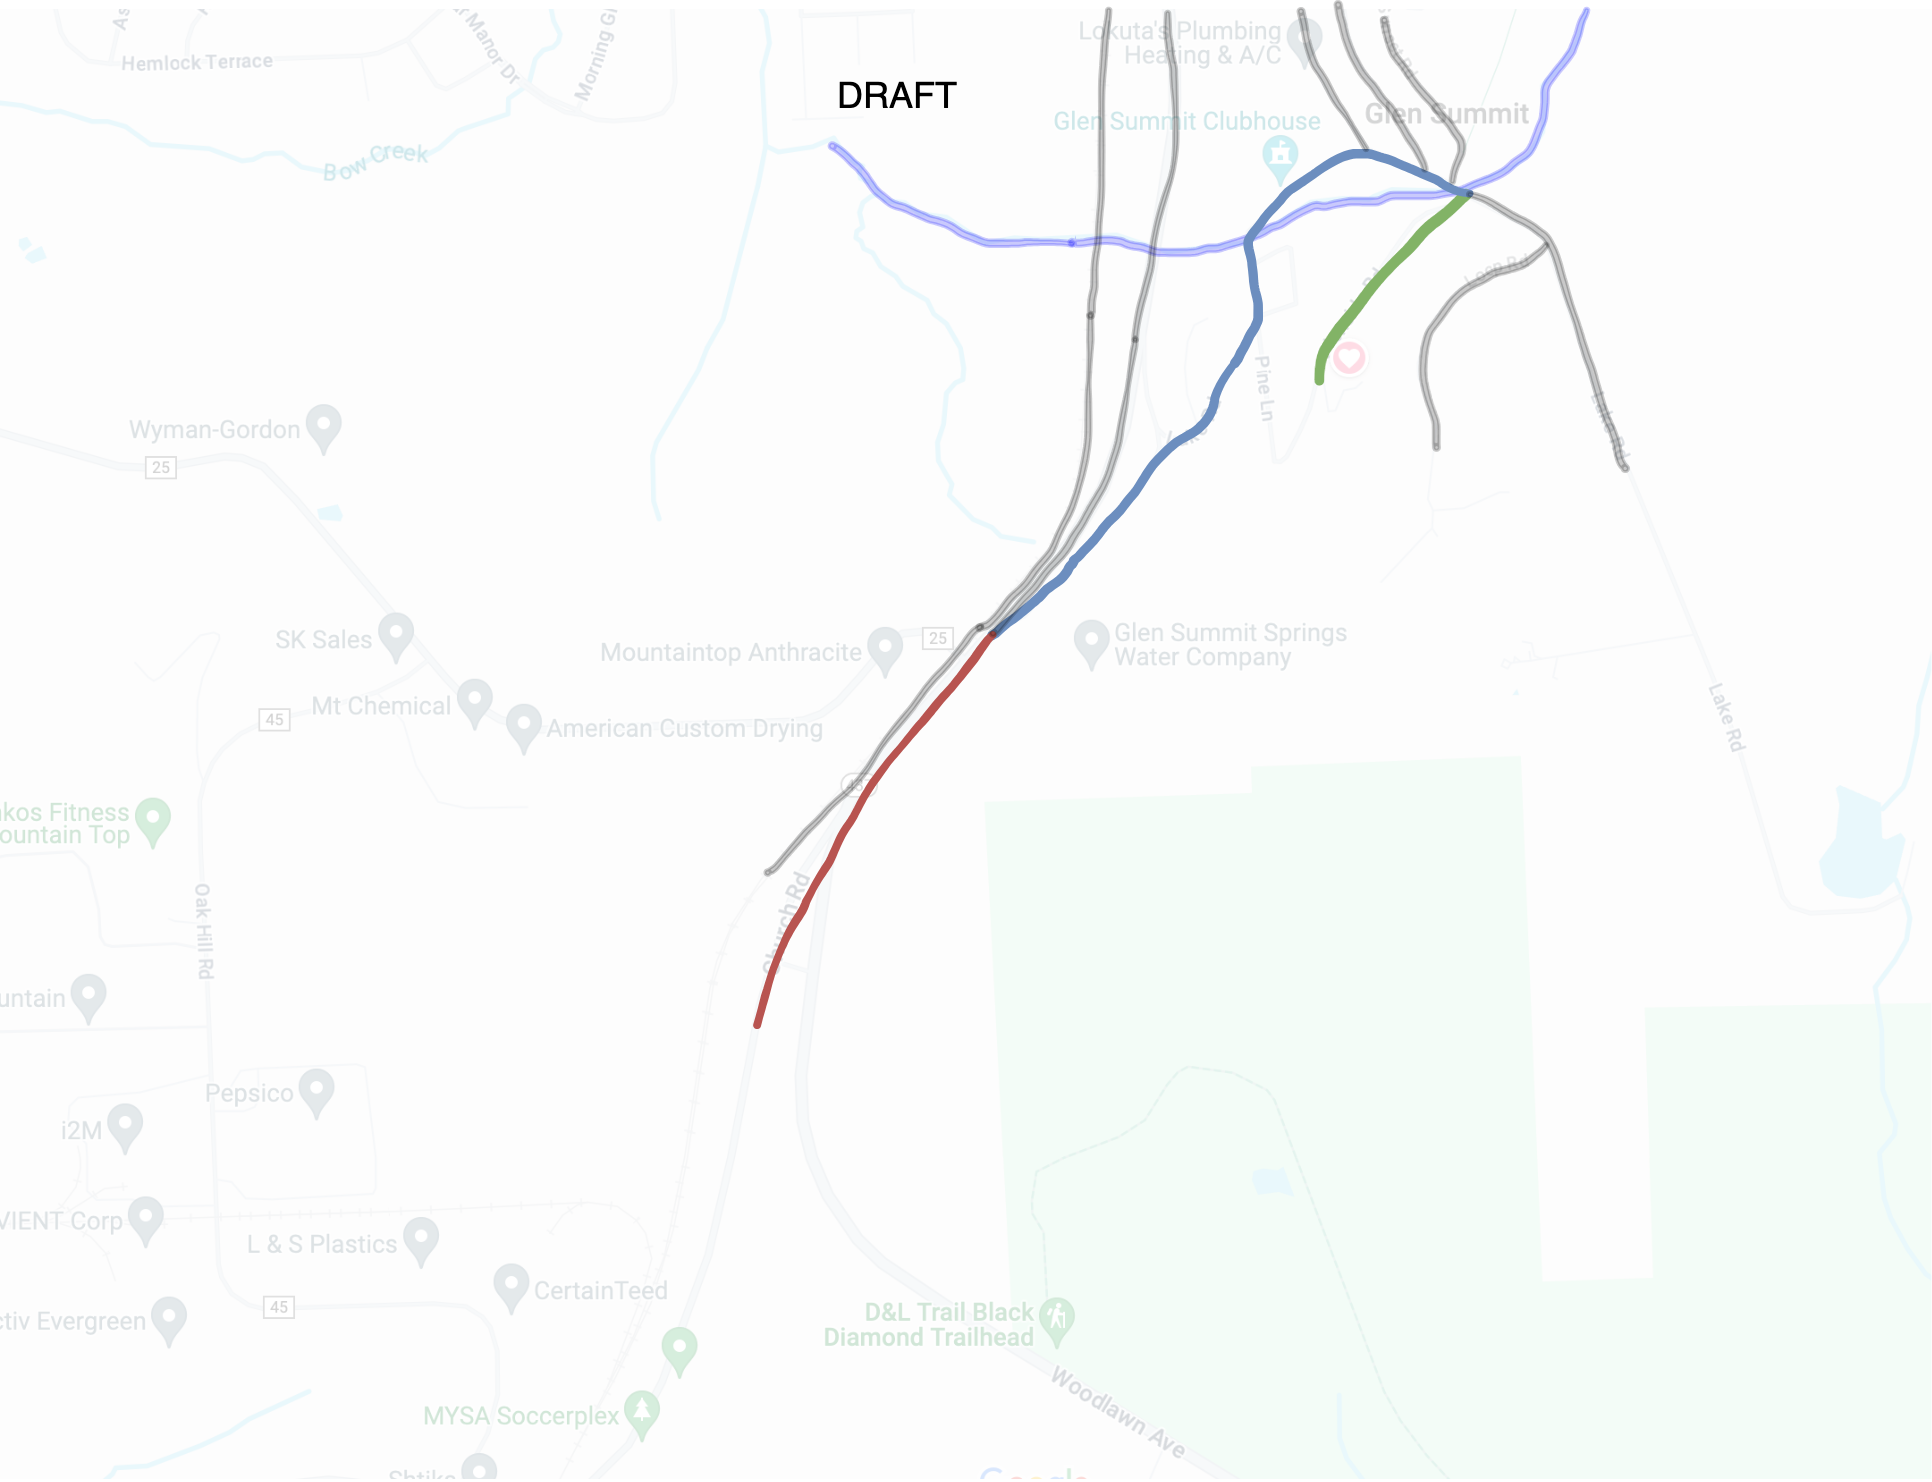
\includegraphics[width=\textwidth]{assets/street-diagram.drawio.png}